\section{引言}
\label{sec:intro}
文本到视频（T2V）生成发展迅速，大规模模型已经可以根据简短文本提示生成视觉效果出色的视频片段 \cite{zheng2024open, yang2024cogvideox, chen2024videocrafter2, wang2025wan}。然而，一个关键问题仍未解决：即使视觉质量很高，当前最先进的 T2V 系统也经常违反基本物理常识。物体可能瞬移、忽略重力，或彼此穿透，从而违背现实世界的物理规律。近期评测 \cite{meng2024towards, bansal2024videophy, Bansal2025} 报告了显著的物理不一致，说明顶尖公开模型仍难以处理需要质量与动量守恒的场景。视觉真实感与物理合理性之间的差距，严重限制了这些模型在机器人、仿真等要求忠实呈现现实动态的领域中的部署。

根本原因之一是 T2V 模型的训练方式和使用方式不匹配。在训练过程中，模型会使用详细、精心制作的描述文本和视频。然而，真实的提示在推理时通常很简短或不明确，从而产生次优的输出 \cite{xue2024phyt2v, cheng2025vpo}。
例如，用户可能输入“\textit{将酒从瓶子中倒入玻璃杯中}”，得到的视频中酒从瓶口流出，但玻璃杯中的液面几乎没有变化（图~\ref{fig:demo} 顶行）。该提示虽然具有较高的语义遵循度（语义得分：5），但物理常识较差（物理得分：3）。关键在于，\emph{手动重写}提示词并加入明确的物理细节，例如“\textit{杯中的液面稳步上升}”，即可生成液体可见累积的物理合理视频（图~\ref{fig:demo} 第二行），并获得满分（语义得分：5，物理得分：5）。这表明当前 T2V 生成器在给定物理感知提示词时\emph{具备}合成物理真实内容的能力；瓶颈在提示词本身。然而，手工提示词工程需要领域专业知识，耗时且难以扩展到多样场景。

现有的自动化方法部分解决了这一差距，但面临着关键的限制。
Promptist \cite{hao2023promptist} 通过监督微调和基于美学奖励的强化学习（RL），自动增强用户给文本到图像模型的输入，但并不面向物理合理性。
早期文本到视频工作使用 GPT-4o 等大语言模型（LLM）通过上下文学习增强提示词；这些方法虽然能提升物理遵循度（例如 GPT-4o 在~\cref{fig:demo} 中达到 PC:5），但可能降低语义保真度（SA:4），且缺少面向视频级物理常识的系统优化。
VPO~\cite{cheng2025vpo} 使用基于偏好的 RL 改进提示，以确保它们无害且准确，但与 Promptist 一样，没有明确解决物理合理性。
最近，PhyT2V 引入了 LLM 引导的迭代式自我完善循环，可在 T2V 提示中实现思维链和“后退”推理，提高对现实世界物理的遵循度，并在分布外场景中超越先前的提示增强器~\cite{xue2024phyt2v}。
虽然 PhyT2V 展示了迭代 LLM 反馈的价值，但它需要多轮提示和复杂的后退机制，限制了其效率。

\begin{figure*}[t]
    \centering
    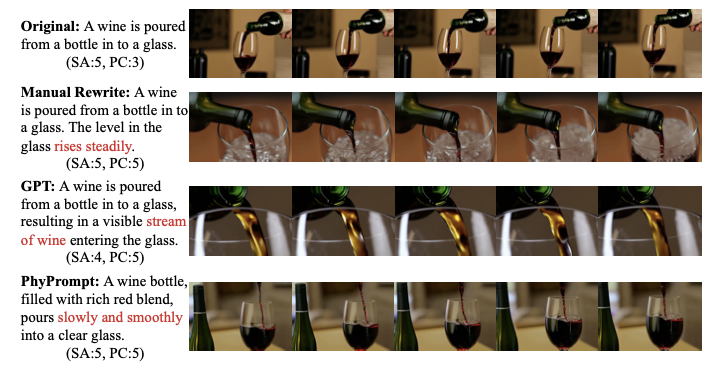
\includegraphics[width=\textwidth]{figures_zh/prompt_demo.png}
    \caption{\textbf{CogVideoX-5B 使用不同提示词生成的视频。} 我们比较原始提示词 \textit{将酒从瓶子中倒入玻璃杯中} 及其三个增强版本：手动重写、GPT-4o 和 PhyPrompt。图中给出了每个结果的语义遵循度（SA）和物理常识（PC）分数。原始提示词未能表现液面上升（PC:3）。手动加入“稳步上升”得到满分（SA:5，PC:5）。GPT-4o 强调“可见的酒流”，但略微降低语义对齐（SA:4，PC:5）。PhyPrompt 自动生成“缓慢而平滑”等物理细节，无需人工干预即可达到手动重写质量（SA:5，PC:5）。}
    \label{fig:demo}
\end{figure*}

为了解决这些限制，我们引入 \textbf{PhyPrompt}，一种利用强化学习训练大语言模型（LLM）的新框架，用于\emph{自动}将用户提示词转换为能够诱导物理真实视频输出的描述，从而在不依赖人工专业知识的情况下达到手工物理感知提示词工程的质量。
我们的方法的特点是两阶段训练流程。
首先，LLM在我们策划的基于 PhyGenBench 的高质量思维链 (CoT) 数据集上进行监督微调 (SFT) \cite{meng2024towards}。
该数据集专门设计用于使LLM能够推理物理现象并将这些考虑因素转化为适合视频生成的描述性文本。
第二阶段，使用组相对策略优化（GRPO）进一步细化经过SFT训练的LLM的提示词生成策略~\cite{guo2025deepseek}，一种 RL 算法，通过对每个查询的多个候选进行采样来有效地探索提示空间，而不需要单独的价值网络。

PhyPrompt 的一个关键创新是受课程培训启发的动态奖励机制 \cite{bengio2009curriculum}。
GRPO 训练由复合奖励信号引导，该信号自适应地平衡生成视频的物理常识及其与用户意图的语义一致性。
在我们的设计中，奖励在训练早期优先考虑语义对齐，随着 LLM 策略逐渐成熟，再逐步将重点转向物理常识。
这种课程式方法确保 LLM 先学会保留用户意图，再专注于增强物理真实性这一更细致的任务。
我们的架构使视频生成器保持冻结状态，仅训练一个轻量级的、与模型无关的重写器，将用户提示转换为物理感知的描述。
这避免了昂贵的生成器微调，并允许一个重写器为多个后端提供服务。

我们在四个尖端生成器上验证了我们的方法：Lavie~\cite{wang2023lavie},VideoCrafter2~\cite{chen2024videocrafter2}、CogVideoX-2B 和 CogVideoX-5B~\cite{wang2024cogvideodex}。
对于每个，我们在用户和生成器之间插入经过训练的 LLM。
对 VideoPhy2 数据集的测试数据集进行的实验表明，重写的提示可以减少物理违规，同时保持视觉质量和语义保真度。
如~\cref{fig:demo} 所示，PhyPrompt 自动生成的提示词可以达到与手工物理感知提示词相同的物理合理性（PC:5）和语义遵循度（SA:5），从而免除了提示词设计中的人工专业知识需求。
这项工作的主要贡献如下：
\begin{itemize}
    \item 我们证明当前的 T2V 生成器在提供物理感知提示时可以生成物理合理的视频，并提出 PhyPrompt，一种新颖的两阶段训练的 LLM 系统。
    \item 我们引入了一种动态的、与时间相关的奖励机制，用于基于强化学习的提示优化，逐步将焦点从语义对齐转移到物理常识，从而促进平衡和有效的学习课程。
      \item 实证验证显示跨多个 T2V 模型的零样本迁移，联合语义遵循度和物理常识增益高达 16.8\%，达到与手工物理感知提示工程相当的质量。
\end{itemize}
